\documentclass[journal,onecolumn]{IEEEtran}
\IEEEoverridecommandlockouts
\usepackage[utf8]{inputenc}
\usepackage[T1]{fontenc}
\usepackage{cite}
\usepackage{amsmath,amssymb}
\usepackage{graphicx}
\usepackage{booktabs}
\usepackage{tabularx}
\usepackage{multirow}
\usepackage{array}
\usepackage{xcolor}
\usepackage{tikz}
\usetikzlibrary{positioning,arrows.meta,fit,calc}
\usepackage{url}
\usepackage[hidelinks]{hyperref}
\newcolumntype{L}[1]{>{\raggedright\arraybackslash}p{#1}}
\newcolumntype{Y}{>{\raggedright\arraybackslash}X}

\begin{document}

\title{Wrecking (Memory) Ball: Processing-in-Memory versus Domain-Specific Accelerators for Irregular Graph Workloads---A Survey}

\author{Vítor~Santos%
\thanks{V.~Santos is with [Affiliation].}}

\markboth{Wrecking (Memory) Ball: PIM versus DSAs for Irregular Graph Workloads}%
{Santos: PIM versus DSAs for Irregular Graph Workloads}

\maketitle

\begin{abstract}
Graph analytics combines poor locality, little computation per byte, and data-dependent control flow. This makes it one of the clearest cases of the memory wall. The architecture literature has answered with two competing philosophies. Processing-in-memory (PIM) moves lightweight compute into or beside DRAM so that data no longer crosses the memory bus. Domain-specific accelerators (DSAs) instead reshape the compute pipeline around the structure of the graph and how it changes over time. This survey examines 30 hardware designs, real-hardware characterization studies, and position papers published between 2015 and 2026, with emphasis on 2021--2026. It compares the two camps on throughput, energy, and memory bandwidth, and makes the evidence base explicit: which baseline each reported number uses, and whether it comes from simulation, field-programmable gate array (FPGA) emulation, or silicon. We find that the camps are not separated by graph size. They are separated by three assumptions: whether the graph changes, how fine-grained accesses are relative to the DRAM burst, and whether inter-unit communication must pass through a host. Every PIM and hybrid hardware design we examined assumes a static graph, whereas the DSA camp has built a lineage of streaming and evolving-graph accelerators. Real PIM hardware delivers less than simulated PIM promises, chiefly because communication between PIM cores is routed through the host. Hybrid designs from 2025--2026 combine PIM bandwidth with DSA-style locality management. We close with the critical-system properties the literature leaves largely unexamined, namely security, dependability, and predictability, and with six open research directions.
\end{abstract}

\begin{IEEEkeywords}
processing-in-memory, near-data processing, domain-specific accelerators, graph analytics, memory wall, survey
\end{IEEEkeywords}

%=====================================================================
\section{Introduction}
%=====================================================================
Graph algorithms such as breadth-first search (BFS), single-source shortest paths (SSSP), PageRank, and subgraph pattern matching underpin applications from social-network analysis to bioinformatics and network security~\cite{ahn2015tesseract,ham2016graphicionado,asquini2025tc}. They map poorly onto conventional processors. Each vertex or edge receives only a few operations, and the next address often depends on the value just loaded, so caches and prefetchers have little to exploit. Tesseract's motivation study illustrates the scale of the mismatch. On a four-socket, 32-core server with 640\,GB/s of memory bandwidth, ideal execution of five graph workloads would need close to 500\,GB/s of mostly random traffic. The authors note that this is beyond what pin-limited systems can deliver for random access~\cite{ahn2015tesseract}. Caches do not close this gap. Piccolo measures that more than 90\% of the bytes a cache fetches during BFS are evicted without ever being used, because one useful 4--8\,B vertex arrives inside a 64\,B burst~\cite{shin2025piccolo}. When the useful fraction is that low, adding bandwidth or capacity to a conventional hierarchy gives diminishing returns. Architects therefore either reduce the distance data travels or increase the useful fraction of each transfer.

Two architectural responses have developed in parallel. The first, \emph{processing-in-memory} (PIM), places compute in the logic layer of 3D-stacked memory, in DRAM buffer chips, beside banks, or inside resistive crossbars. Data then moves over short internal paths instead of the external bus~\cite{ahn2015tesseract,song2018graphr,gomezluna2022prim}. The second, \emph{domain-specific acceleration}, keeps memory conventional and builds specialized pipelines, schedulers, and on-chip storage around the vertex-centric execution model~\cite{ham2016graphicionado,mukkara2018hats,yan2019graphdyns}. A 2019 survey of graph accelerators concluded that there was ``not an absolute winner'' across preprocessing, parallel computation, and runtime scheduling~\cite{gui2019survey}. Since then the field has changed substantially. Commercial PIM hardware (UPMEM) has been characterized on real workloads~\cite{gomezluna2022prim,barkhordar2025alphapim}. DSAs have extended to streaming and evolving graphs~\cite{rahman2021jetstream,zhao2022tdgraph,gao2023mega}. A new class of hybrid designs has appeared~\cite{shin2025piccolo,shin2025fala,yenimol2026cograf}. This survey asks:

\begin{quote}\itshape
For irregular graph workloads, how do PIM architectures and discrete DSAs trade off throughput, energy efficiency, and effective memory bandwidth, and which workload and system assumptions decide when each is better?
\end{quote}

Four sub-questions structure the analysis. \textbf{SQ1} asks which bottleneck each camp attacks and how its design lineage has evolved. \textbf{SQ2} asks what the reported results support once baselines and evaluation substrates are made explicit. \textbf{SQ3} asks which assumptions decide which camp is better. \textbf{SQ4} asks how the camps differ on security, dependability, and predictability. Our contributions are:
(i)~a placement-based taxonomy of 30 works by where the compute sits in the memory hierarchy (Section~\ref{sec:background});
(ii)~a camp-by-camp review that follows each design lineage and reports every headline number together with its baseline (Sections~\ref{sec:pim}--\ref{sec:hybrid});
(iii)~a comparative analysis showing that graph mutability, access granularity, and host-mediated communication explain the published evidence better than graph size does (Section~\ref{sec:analysis});
and (iv)~an assessment of critical-system properties and open challenges (Sections~\ref{sec:critical}--\ref{sec:open}).
Graph neural network accelerators, GPU-only systems, and near-storage graph processing are outside our scope.

The remainder of the paper is organized as follows. Section~\ref{sec:background} introduces the workload model, the placement taxonomy, and our survey method. Sections~\ref{sec:pim} and~\ref{sec:dsa} review the PIM and DSA lineages, and Section~\ref{sec:hybrid} covers the hybrid designs that combine them. Section~\ref{sec:analysis} compares the camps on throughput, energy, bandwidth, evidence quality, cost, and the assumptions that decide between them. Section~\ref{sec:critical} evaluates security, dependability, and predictability, Section~\ref{sec:open} lists open challenges, and the final section summarizes our conclusions.

%=====================================================================
\section{Background and Survey Method}\label{sec:background}
%=====================================================================
\subsection{Graph workloads}
Most surveyed designs adopt the vertex-centric model. In each iteration, active vertices read their edges, generate updates for their neighbours (\emph{scatter} or \emph{push}), and the updates are reduced into destination properties (\emph{apply})~\cite{ham2016graphicionado,yenimol2026cograf}. Graphs are typically stored in compressed sparse row (CSR) or column form, which favours sequential edge streaming but makes insertion expensive. Coordinate (COO) lists are easy to append to but harder to traverse~\cite{asquini2025tc}. Traversal workloads (BFS, SSSP) activate a small and shifting \emph{frontier} each iteration. PageRank-style workloads touch every vertex. Graph mining instead consists largely of set intersections and unions over neighbour lists~\cite{besta2021sisa}. Two properties recur in every design we survey. First, vertex properties are small (4--8\,B) compared with the 64\,B DRAM burst, so a cache line fetched for one vertex is mostly wasted~\cite{shin2025piccolo}. Second, real-world degree distributions are skewed, which unbalances both partitions and crossbar mappings~\cite{zheng2020spara,cai2024pimpam}.

Two execution-model choices recur and affect hardware design directly. The first is \emph{synchronization}. Bulk-synchronous designs process all active vertices of an iteration before starting the next, as Graphicionado does~\cite{ham2016graphicionado}. Asynchronous and event-driven designs propagate updates as soon as they are produced. JetStream builds on such an event-driven accelerator, which its authors report achieved up to $6\times$ over a bulk-synchronous design~\cite{rahman2021jetstream}, and GraphQ's multi-node model tolerates bounded staleness~\cite{zhuo2019graphq}. The second is \emph{direction}. Push-based execution writes updates into neighbours and therefore creates scattered writes that PIM can absorb in place. Pull-based execution reads from neighbours and does not map as naturally onto PIM. CoGraf, for example, evaluates push-only variants for this reason~\cite{yenimol2026cograf}. GraphDynS summarizes the resulting difficulties as three irregularities: \emph{workload} irregularity (unequal edges per thread), \emph{traversal} irregularity (unpredictable edges per iteration, with atomic conflicts when many edges update one vertex), and \emph{update} irregularity (the set of updated and activated vertices changes every iteration, yet all vertices are checked)~\cite{yan2019graphdyns}. Reported metrics vary across papers. Most report speedup and energy relative to a baseline; some report traversed edges per second (TEPS) or TEPS per watt~\cite{lee2022graphwave}. This variety is one reason why direct comparison across camps is difficult.

\subsection{Where does the compute sit?}
We classify designs by the level of the memory hierarchy at which graph computation executes (Fig.~\ref{fig:placement}). \emph{On-chip DSAs} sit on the processor side of the memory bus, either as stand-alone accelerators or as units attached to cores~\cite{ham2016graphicionado,mukkara2018hats,zhao2022tdgraph}. \emph{Processing-near-memory} (PnM) places programmable cores or fixed-function units in a 3D-stack logic layer~\cite{ahn2015tesseract,zhuo2019graphq}, in a DIMM buffer chip~\cite{talati2022ndminer}, or beside each DRAM bank, as in UPMEM~\cite{gomezluna2022prim}. \emph{Fine-grained} or \emph{bank-level} PIM adds simple column-wide ALUs inside banks~\cite{yenimol2026cograf,shin2025fala}. \emph{Processing-using-memory} with resistive crossbars performs analog sparse matrix--vector multiplication in the memory array itself~\cite{song2018graphr,zheng2020spara,challapalle2020gaasx}. The deeper the placement, the higher the available internal bandwidth. Deeper placement also brings greater restrictions on precision, programmability, and communication.

\begin{figure}[t]
\centering
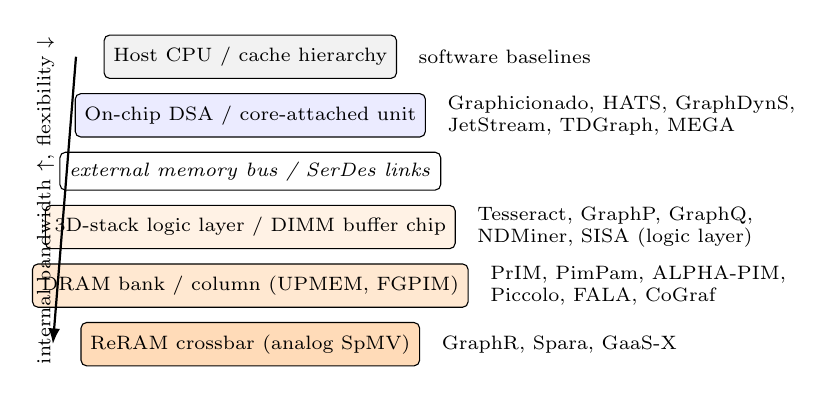
\begin{tikzpicture}[
  lvl/.style={draw, rounded corners=2pt, minimum width=3.0cm, minimum height=0.55cm, font=\scriptsize, align=center},
  ex/.style={font=\scriptsize, align=left, anchor=west},
  node distance=0.18cm]
\node[lvl, fill=gray!10] (host) {Host CPU / cache hierarchy};
\node[lvl, fill=blue!8, below=of host] (dsa) {On-chip DSA / core-attached unit};
\node[lvl, fill=white, below=of dsa, minimum height=0.35cm] (bus) {\textit{external memory bus / SerDes links}};
\node[lvl, fill=orange!10, below=of bus] (logic) {3D-stack logic layer / DIMM buffer chip};
\node[lvl, fill=orange!18, below=of logic] (bank) {DRAM bank / column (UPMEM, FGPIM)};
\node[lvl, fill=orange!28, below=of bank] (xbar) {ReRAM crossbar (analog SpMV)};
\node[ex, right=0.15cm of host] {software baselines};
\node[ex, right=0.15cm of dsa] {Graphicionado, HATS, GraphDynS,\\ JetStream, TDGraph, MEGA};
\node[ex, right=0.15cm of logic] {Tesseract, GraphP, GraphQ,\\ NDMiner, SISA (logic layer)};
\node[ex, right=0.15cm of bank] {PrIM, PimPam, ALPHA-PIM,\\ Piccolo, FALA, CoGraf};
\node[ex, right=0.15cm of xbar] {GraphR, Spara, GaaS-X};
\draw[-{Latex[length=2mm]}, thick] ([xshift=-0.35cm]host.west) -- node[left, font=\scriptsize, align=center, rotate=90, anchor=south] {internal bandwidth $\uparrow$, flexibility $\downarrow$} ([xshift=-0.35cm]xbar.west);
\end{tikzpicture}
\caption{Taxonomy by compute placement. The deeper the compute sits, the more internal bandwidth it can use, at the cost of precision, programmability, and direct communication between units.}
\label{fig:placement}
\end{figure}

\subsection{Survey method}
The corpus was assembled through web searches targeting the ACM Digital Library, IEEE Xplore, arXiv, dblp, and author pages, and each entry was verified against a publisher, dblp, institutional, or author record. The search was focused on ISCA, MICRO, HPCA, ASPLOS, and DSN, with 2021--2026 as the primary window. A design was included if it proposes or evaluates PIM, near-data, or domain-specific hardware for graph analytics, traversal, or mining. Seminal pre-2021 designs that later work compares against are included as background. All but two included works were analysed in full text, and every reported number was taken from the paper itself. The exceptions, MGX and NDMiner, are cited only for claims stated in their abstracts. FPGA designs are represented by one reference point (ReGraph~\cite{chen2022regraph}), because our comparison concerns ASIC and PIM design philosophies. Two software systems, CommonGraph~\cite{afarin2023commongraph} and Glign~\cite{yin2023glign}, are cited as algorithmic context and not counted as hardware. Table~\ref{tab:corpus} summarizes the corpus. Two caveats apply. First, PIM designs outnumber DSAs. We read this as partly a finding in its own right: graph PIM is the more active design space at the target venues since 2021, whereas many graph DSAs predate 2021. Second, absence claims in this paper mean ``not found in our search'' over the stated venues and years, not proof that no such work exists.

\emph{Comparison rule.} The surveyed papers report speedups against single-threaded CPUs, multi-threaded frameworks, GPUs, or prior accelerators, measured on different datasets and on different substrates (cycle-level simulation, FPGA emulation, or silicon). We therefore never place two numbers side by side unless both their baseline class and their substrate match, and every number in Table~\ref{tab:designs} is stated together with its baseline.

\begin{table}[t]
\caption{Surveyed corpus by camp and evaluation substrate}
\label{tab:corpus}
\centering\scriptsize
\begin{tabularx}{\columnwidth}{@{}L{1.55cm}YL{1.15cm}@{}}
\toprule
Camp / class & Works & Substrate \\
\midrule
PIM, 3D-stack / buffer & Tesseract~\cite{ahn2015tesseract}, GraphP~\cite{zhang2018graphp}, GraphQ~\cite{zhuo2019graphq}, SISA~\cite{besta2021sisa}, SynCron~\cite{giannoula2021syncron}, NDMiner~\cite{talati2022ndminer} & simulation \\
PIM, analog ReRAM & GraphR~\cite{song2018graphr}, Spara~\cite{zheng2020spara}, GaaS-X~\cite{challapalle2020gaasx} & sim.\ + SPICE \\
PIM, real hardware & PrIM~\cite{gomezluna2022prim}, PimPam~\cite{cai2024pimpam}, ALPHA-PIM~\cite{barkhordar2025alphapim}, TC on UPMEM~\cite{asquini2025tc} & UPMEM silicon \\
DSA, static & Graphicionado~\cite{ham2016graphicionado}, HATS~\cite{mukkara2018hats}, GraphDynS~\cite{yan2019graphdyns}, GraphWave~\cite{lee2022graphwave}, ReGraph~\cite{chen2022regraph} & sim.; FPGA \\
DSA, dynamic & JetStream~\cite{rahman2021jetstream}, TDGraph~\cite{zhao2022tdgraph}, MEGA~\cite{gao2023mega} & simulation \\
Hybrid & Piccolo~\cite{shin2025piccolo}, FALA~\cite{shin2025fala}, CoGraf~\cite{yenimol2026cograf} & sim.; FPGA emul. \\
Security / position & MGX~\cite{hua2022mgx}, IMPACT~\cite{bostanci2025impact}, PiD security~\cite{yuksel2026pid}, Kim \& Kim~\cite{kim2020dynamic} & mixed \\
Software context & CommonGraph~\cite{afarin2023commongraph}, Glign~\cite{yin2023glign} & CPU \\
\bottomrule
\end{tabularx}
\end{table}

%=====================================================================
\section{Processing-in-Memory for Graphs}\label{sec:pim}
%=====================================================================
\subsection{3D-stacked PIM: a decade-long fight with communication}
Tesseract established the template for graph PIM~\cite{ahn2015tesseract}. Each vault of a Hybrid Memory Cube (HMC) receives a simple in-order core. Instead of reading remote data, Tesseract moves computation to the data through \emph{remote function calls}. Non-blocking calls hide latency and make updates atomic without software locks. Two specialized prefetchers, guided by hints from the programming interface, keep the simple cores fed. With 16 cubes, the cores see 8\,TB/s of aggregate internal bandwidth, compared with 640\,GB/s for the baseline server. Tesseract reports roughly a $10\times$ performance gain and an 87\% energy reduction over that baseline on graphs of four to seven million vertices~\cite{ahn2015tesseract}. The key property is that bandwidth scales with memory capacity: adding cubes adds both storage and compute.

The follow-on work shows where that scaling breaks. Tesseract's vertex-programming model distributes edges so that each cross-cube edge generates a remote message over SerDes links whose bandwidth is far below the cubes' aggregate internal bandwidth. GraphP therefore makes data organization a first-order concern. Its ``source-cut'' partitioning sends one update per replica instead of one per edge, giving a $1.7\times$ speedup and 89\% energy saving \emph{over Tesseract} in cycle-accurate simulation~\cite{zhang2018graphp}. GraphQ goes further by reordering vertex processing so that inter-cube messages are batched, structured, and overlapped with computation. It uses heterogeneous cores for different access types. Because the bandwidth between nodes is lower still than that between cubes, it also adds a hybrid execution model in which nodes perform extra local computation during inter-node communication. This model is valid for asynchronous iterative algorithms that tolerate bounded stale values~\cite{zhuo2019graphq}. GraphQ reports $3.3\times$ on average ($13.9\times$ maximum) and 81\% energy saving over Tesseract in zSim~\cite{zhuo2019graphq}. Its widely quoted $98.34\times$ figure compares a four-node GraphQ with a \emph{single node using a conventional memory hierarchy}. It is evidence of capacity-proportional scaling, not a gain over prior PIM~\cite{zhuo2019graphq}. Across the lineage, each improvement removes a communication irregularity that the previous design left in place. Raw compute capability barely changes.

\subsection{Analog resistive RAM (ReRAM) PIM: trading precision for energy}
GraphR takes a different route. If a vertex program can be expressed as sparse matrix--vector multiplication (SpMV), small graph blocks can be programmed into ReRAM crossbars and processed in the analog domain~\cite{song2018graphr}. GraphR reports a geometric-mean speedup of $16.01\times$ (maximum $132.67\times$) and $33.82\times$ energy saving over a CPU baseline, $1.69$--$2.19\times$ speedup over a GPU, and $1.16$--$4.12\times$ speedup over a PIM architecture~\cite{song2018graphr}. Its weakness is sparsity. Real graphs leave most crossbar cells holding zeros, and because activations depend on the input, many cycles do no useful work. Spara maps source vertices randomly to wordlines and destination vertices consecutively to bitlines, and adds a bank-parallel architecture that keeps crossbars densely occupied. It reports $8.21\times$ and $5.01\times$ performance and $8.97\times$ and $5.68\times$ energy savings over GraphR and GraphSAR, respectively. Its lightweight reordering costs only 3.9--6.6\% extra preprocessing time on the largest graph evaluated~\cite{zheng2020spara}. Spara also illustrates a recurring trade-off in the analog class: mapping quality depends on vertex ordering, so the hardware's efficiency depends on software preprocessing that must be repeated whenever the graph changes. GaaS-X supports sparse formats natively, using content-addressable crossbars to avoid sparse-to-dense conversion and redundant writes. It reports $7.7\times$ and $2.4\times$ performance and $22\times$ and $5.7\times$ energy savings over GraphR and GRAM~\cite{challapalle2020gaasx}. The class as a whole is restricted to SpMV-expressible kernels, and its precision is bounded by analog-to-digital conversion. GraphR argues that iterative graph algorithms tolerate this imprecision~\cite{song2018graphr}, a claim we revisit in Section~\ref{sec:critical}.

\subsection{Set-centric mining and synchronization infrastructure}
Graph mining stresses PIM differently from traversal. SISA observes that set intersections and unions dominate many mining algorithms. It exposes them as instruction-set architecture (ISA) extensions and maps them to two kinds of PIM: in-DRAM bulk bitwise operations for the dense neighbour sets of high-degree vertices, and logic-layer cores for the sparse integer arrays of low-degree vertices. Between 5\% and 30\% of the largest neighbourhoods are stored as bitvectors, and the rest as integer arrays, so the representation itself adapts to degree skew. SISA reports more than $10\times$ speedup over the Bron--Kerbosch maximal-clique algorithm~\cite{besta2021sisa}. SISA is notable because it combines two PIM placements, in-DRAM and logic layer, in one design, routing work by degree. The hybrids of Section~\ref{sec:hybrid} generalize this idea to the host-versus-memory split. NDMiner places set-operation units in the DRAM buffer chip, together with hardware that elides loads ruled out by symmetry-breaking constraints. Its abstract reports $6.4\times$ and $2.5\times$ over software and hardware baselines~\cite{talati2022ndminer}. Any parallel PIM design also needs synchronization without cache coherence. SynCron provides near-data synchronization engines and reports $1.27\times$ (high contention) and $1.35\times$ (real applications) improvements over prior schemes~\cite{giannoula2021syncron}.

\subsection{Real hardware: the UPMEM reality check}
Until recently, PIM evidence came from simulation or, at best, simplified hardware prototypes~\cite{gomezluna2022prim}. UPMEM's commercial PIM DIMMs changed this. Each DRAM processing unit (DPU) is a 350\,MHz in-order core with exclusive access to a 64\,MB bank and a 64\,KB scratchpad. The decisive constraint is that \emph{DPUs cannot communicate directly}: all inter-DPU data moves through the host CPU over the memory bus~\cite{gomezluna2022prim}. The PrIM characterization found that a 2,556-DPU system beats a modern CPU by $93.0\times$ on average on the 13 benchmarks that avoid heavy inter-DPU synchronization (a 640-DPU system, by $27.9\times$). The smaller system is nevertheless slower than a GPU on most benchmarks~\cite{gomezluna2022prim}. BFS is one of the benchmarks that does not avoid it. After every BFS iteration the host merges the per-DPU frontiers sequentially and redistributes them, so adding DPUs barely reduces synchronization time~\cite{gomezluna2022prim}.

Graph studies on the same platform confirm the pattern. PimPam achieves a $22.5\times$ average speedup over the GraphPi CPU framework for pattern matching~\cite{cai2024pimpam}. Its four key optimizations are telling: load-aware task assignment, space-efficient parallel partitioning that fits each DPU's share of the graph into its 64\,MB bank, adaptive multithreading, and dynamic bitmaps. Every one of them works around a constraint of the platform (limited per-core memory, no inter-core communication, weak in-order cores) rather than exploiting a property of the graph~\cite{cai2024pimpam}. ALPHA-PIM reformulates BFS, SSSP, and personalized PageRank as sparse matrix--sparse vector products. It finds that the best data partitioning depends on input-vector density and dataset. It measures DPU compute utilization of 18.5\% within the kernel but only 5\% end to end for BFS, which is still far above the 0.01--0.05\% it measures on CPU and GPU. The authors call for better direct memory access (DMA) engines, more instruction-level parallelism, and direct interconnects between PIM cores~\cite{barkhordar2025alphapim}. A 2025 workshop paper on triangle counting uses vertex coloring to avoid inter-DPU communication, reservoir sampling to fit within bank capacity, and a Misra--Gries summary to handle high-degree vertices. It nevertheless finds that UPMEM loses to CPU (CSR) and GPU implementations on static graphs~\cite{asquini2025tc}. PIM wins only when updates arrive as appended COO batches that would force the CPU to rebuild its CSR. The real-hardware evidence therefore narrows the simulation narrative: the bandwidth benefit is real, but host-mediated communication caps it for exactly the frontier-driven traversals that motivate graph PIM.

%=====================================================================
\section{Domain-Specific Accelerators}\label{sec:dsa}
%=====================================================================
\subsection{Static-graph pipelines}
Graphicionado is the reference graph DSA~\cite{ham2016graphicionado}. It maps the vertex-programming model onto a reconfigurable pipeline specialized for vertex and edge datatypes. The key memory-side change moves random destination-vertex updates from off-chip DRAM to a large on-chip scratchpad. Scaling the pipeline is not simply a matter of replication: replicated streams that read and write the same scratchpad locations are serialized. Graphicionado therefore splits the pipeline into a source-oriented and a destination-oriented portion, replicates each separately, and routes edges between them through a crossbar keyed by destination vertex~\cite{ham2016graphicionado}. Graphicionado reports a $1.76$--$6.54\times$ speedup and $50$--$100\times$ lower energy than a 32-thread software framework on a 16-core Xeon, evaluated with register-transfer level (RTL) synthesis and DRAMSim2~\cite{ham2016graphicionado}. HATS takes a different approach. It argues that locality exists in real graphs' community structure but is hard to predict ahead of time, and that offline reordering costs more than it saves. HATS therefore implements bounded depth-first scheduling (BDFS) as a small hardware unit beside each core. BDFS restricts each core to explore a small, well-connected region depth-first up to a bounded depth, which improves temporal locality on graphs with community structure. The paper contrasts a vertex-ordered engine (VO-HATS) with BDFS-HATS. On PageRank Delta over the uk-2002 graph, the two improve performance by $1.8\times$ and $2.7\times$, respectively. In zsim, BDFS reduces main-memory accesses by up to $2.4\times$ (30\% on average) without any preprocessing~\cite{mukkara2018hats}. HATS is significant for this survey because it shows that a DSA can recover locality \emph{online}. That ability matters again for dynamic graphs, where offline reordering is never finished. HATS is also cheap: it requires 0.14\,mm$^2$ and 72\,mW at 65\,nm, negligible next to a general-purpose core~\cite{mukkara2018hats}. This shows that locality-aware scheduling does not require a stand-alone accelerator. TDGraph's per-core engines follow the same approach, and TDGraph uses HATS as one of its baselines~\cite{zhao2022tdgraph}. GraphDynS identifies data-dependent behaviour as the root of the irregularity. Its Dispatching/Processing programming model decouples the datapath so that data dependencies can be extracted at runtime. A data-aware scheduler then uses those dependencies to schedule workloads, data accesses, and computations on the fly, which the authors show addresses all three irregularities. The design is implemented in RTL and evaluated with five algorithms on six real-world and five synthetic graphs~\cite{yan2019graphdyns}. It reports $4.4\times$ speedup and $11.6\times$ less energy than a GPGPU solution \emph{using half the memory bandwidth}, and $1.9\times$ speedup with $1.8\times$ less energy than a prior graph accelerator at \emph{equal} bandwidth~\cite{yan2019graphdyns}. GraphDynS thus attacks irregularity at its source, whereas Graphicionado and HATS work around its effects. GraphWave, aimed at edge devices, assigns one functional unit to every vertex and optimizes the on-chip multicast network. It reaches 97.8\,GTEPS at 63.94\,GTEPS/W in gate-level simulation, but the supported graph size is bounded by the number of on-chip units~\cite{lee2022graphwave}.

\subsection{An FPGA reference point}
ReGraph shows what happens when a DSA is given PIM-like bandwidth through a High Bandwidth Memory (HBM) package~\cite{chen2022regraph}. On an Alveo U280 with 32 HBM channels (460\,GB/s), monolithic pipeline designs run out of logic resources long before they can saturate the channels. ReGraph therefore classifies partitions as dense or sparse and pairs ``Little'' pipelines for the dense partitions with ``Big'' pipelines for the sparse, poorly local ones, using model-guided scheduling. It reports $1.6$--$5.9\times$ performance and $12\times$ resource efficiency over prior FPGA designs~\cite{chen2022regraph}. ReGraph is also the one design in our DSA set that runs on real hardware end to end, so its numbers include effects, such as routing and resource limits, that simulation typically omits. The lesson for our comparison is that once external bandwidth is plentiful, the DSA bottleneck moves to the number of pipelines that fit and to how heterogeneous the partitions are.

\subsection{The temporal lineage: streaming and evolving graphs}
The most distinctive post-2021 DSA development concerns graphs that change. JetStream extends the event-driven GraphPulse accelerator to handle edge additions, deletions, and updates. It reuses prior query results and confines recomputation to affected vertices. It supports both accumulative algorithms (e.g., PageRank) and monotonic ones (e.g., SSSP, where deletions can invalidate previously settled values), and limits memory accesses to the affected subset of vertices. It reports 90\% less computation time than a cold-start recomputation and about $18\times$ speedup over the KickStarter and GraphBolt software frameworks, with larger gains at smaller batch sizes~\cite{rahman2021jetstream}. The batch-size dependence matters for latency-sensitive uses: the smaller the update batch, the more an incremental accelerator gains over recomputation. TDGraph couples a topology-driven engine to each core of a many-core processor. The engine sits between the core and its private L2 cache and operates on virtual addresses through the core's translation lookaside buffer (TLB), so it shares the conventional memory hierarchy instead of replacing it~\cite{zhao2022tdgraph}. It starts incremental computation from the vertices touched by updates and prefetches along the topology, so that propagations from many updates are merged. In a simulated 64-core system it reports $7.1$--$21.4\times$ over a software streaming system and $4.6$--$12.7\times$ over HATS at 0.73\% area cost~\cite{zhao2022tdgraph}. MEGA targets \emph{evolving} graphs, where one query must be evaluated across many snapshots. It builds on the CommonGraph software insight that converting deletions into additions against a common base graph avoids expensive deletions~\cite{afarin2023commongraph}, and adds batch-oriented execution so that snapshots sharing update batches are evaluated together. MEGA reports $24$--$120\times$ over CommonGraph and $4.08$--$5.98\times$ over JetStream~\cite{gao2023mega}. Taken together, the three designs show the DSA camp moving from single-snapshot streaming, to topology-aware incremental propagation, to multi-snapshot evolution. In each step, the accelerator's control logic grows to track what changed, while the memory system stays conventional. Concurrent queries over a shared graph raise a related problem of misaligned traversals. It has so far been addressed in software by Glign, which aligns concurrent traversals to recover shared locality~\cite{yin2023glign}.

\begin{figure}[t]
\centering
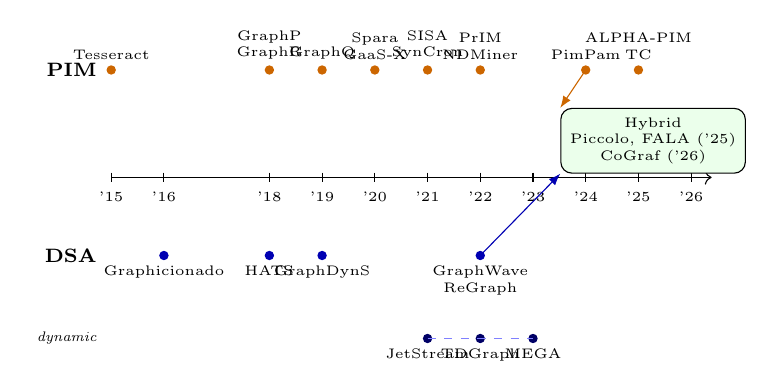
\begin{tikzpicture}[x=0.62cm,y=0.62cm,
  ev/.style={font=\tiny, align=center, inner sep=1pt},
  dot/.style={circle, fill, inner sep=1.2pt}]
\draw[->] (0,0) -- (12.3,0);
\foreach \y/\lab in {2015/15,2016/16,2018/18,2019/19,2020/20,2021/21,2022/22,2023/23,2024/24,2025/25,2026/26}{
  \pgfmathsetmacro{\xx}{(\y-2015)*1.08}
  \draw (\xx,0.1) -- (\xx,-0.1) node[below, font=\tiny] {'\lab};}
% PIM track
\node[font=\scriptsize\bfseries, anchor=east] at (-0.1,2.2) {PIM};
\foreach \x/\t in {0/Tesseract, 3.24/GraphP\\GraphR, 4.32/GraphQ, 5.40/Spara\\GaaS-X, 6.48/SISA\\SynCron, 7.56/PrIM\\NDMiner, 9.72/PimPam}{
  \node[dot, orange!80!black] at (\x,2.2) {}; \node[ev, above] at (\x,2.35) {\t};}
% DSA track
\node[font=\scriptsize\bfseries, anchor=east] at (-0.1,-1.6) {DSA};
\foreach \x/\t in {1.08/Graphicionado, 3.24/HATS, 4.32/GraphDynS, 7.56/GraphWave\\ReGraph}{
  \node[dot, blue!70!black] at (\x,-1.6) {}; \node[ev, below] at (\x,-1.75) {\t};}
% dynamic branch
\node[font=\tiny\itshape, anchor=east] at (-0.1,-3.3) {dynamic};
\foreach \x/\t in {6.48/JetStream, 7.56/TDGraph, 8.64/MEGA}{
  \node[dot, blue!40!black] at (\x,-3.3) {}; \node[ev, below] at (\x,-3.45) {\t};}
\draw[blue!50, dashed] (6.48,-3.3) -- (8.64,-3.3);
% hybrid convergence
\node[draw, rounded corners, fill=green!8, font=\tiny, align=center] (hy) at (11.1,0.75) {Hybrid\\Piccolo, FALA ('25)\\CoGraf ('26)};
\draw[-{Latex[length=1.5mm]}, orange!80!black] (9.72,2.2) -- (hy.north west);
\draw[-{Latex[length=1.5mm]}, blue!70!black] (7.56,-1.6) -- (hy.south west);
\node[dot, orange!80!black] at (10.8,2.2) {}; \node[ev, above] at (10.8,2.35) {ALPHA-PIM\\TC};
\end{tikzpicture}
\caption{Design lineages. Both camps converge into hybrid designs in 2025--2026, but only the DSA track has a dynamic-graph branch.}
\label{fig:lineage}
\end{figure}

%=====================================================================
\section{Convergence: Hybrid Designs}\label{sec:hybrid}
%=====================================================================
Three recent designs reject the binary framing. They argue that a pure DSA wastes bandwidth on coarse DRAM bursts, and that a pure PIM cannot exploit the data reuse that tiling provides~\cite{shin2025piccolo,shin2025fala}. Piccolo starts from a DSA, using GraphDynS as its baseline accelerator~\cite{shin2025piccolo}. It observes that the 64\,B DDR burst is an order of magnitude larger than a 4--8\,B vertex property, so that in BFS more than 90\% of fetched data is evicted unused. Instead of placing arithmetic units in memory, Piccolo adds \emph{fine-grained in-memory scatter-gather}, so that tiles fetch only useful vertex data. It reports a $1.62\times$ geometric-mean speedup (up to $3.28\times$) over its strongest baseline, a cache-based GraphDynS, and up to 59.7\% energy reduction, with the in-memory mechanism validated by FPGA emulation and performance measured with Ramulator-based cycle-level simulation~\cite{shin2025piccolo}. FALA, from the same group, combines three mechanisms. A lightweight unit in each HBM2 bank performs the reduce phase of the vertex program. A fine-grained column-access mechanism fetches several non-contiguous 8\,B columns from one open row. A locality-aware offloading policy routes accesses to the host cache or to PIM according to their locality, which follows from skewed degree distributions. It reports $1.56\times$ speedup and 35.3\% energy reduction (geometric mean) over the best prior design, evaluated against Piccolo, PEI, and GraphPIM~\cite{shin2025fala}. CoGraf targets fine-grained PIM (FGPIM) for push-based vertex programs. A tuple-based last-level cache coalesces updates to match DRAM column parallelism. Once the update phase is accelerated, the apply phase becomes the bottleneck, which CoGraf addresses with bank-parallel predicated PIM instructions. It reports $4.4\times$/$9.8\times$ speedups over a state-of-the-art non-PIM baseline on HBM2/DDR4 and 88\%/94\% DRAM energy reduction. These figures are measured over the region of interest, not end to end~\cite{yenimol2026cograf}.

The hybrids also respond to a cost argument. Piccolo deliberately avoids placing arithmetic units in DRAM, stating that doing so is expensive and that supporting multiple operation types there is impractical~\cite{shin2025piccolo}. FALA notes that commercial DRAM-PIM products with parallel arithmetic units have been reported to add up to 50\% area overhead to the DRAM die. It also points out that many earlier PIM proposals assumed separate logic dies with serial interconnects, which do not map onto monolithic DRAM-PIM~\cite{shin2025fala}. The hybrids therefore place the minimum function in memory (scatter-gather, fine-grained column selection, simple reduction) and keep control and reuse on the processor side.

The hybrids matter for the research question in two ways. First, they show that the two camps are converging. The DSA side contributes cache- and tile-level locality management, and the PIM side contributes internal bandwidth and fine access granularity. The hybrids also inherit a limitation from each camp. From the DSA side, they inherit dependence on tiling and cache reuse, which is strongest when the working set is stable. From the PIM side, they inherit the need for modified memory parts, even if the modification is small. Second, all three keep the static-graph assumption: none of their full texts mentions dynamic, streaming, or evolving graphs~\cite{shin2025piccolo,shin2025fala,yenimol2026cograf}.

%=====================================================================
\section{Comparative Analysis}\label{sec:analysis}
%=====================================================================
\subsection{Throughput}
Both camps report large throughput gains, but against baselines that cannot be compared. The PIM gains are largest against conventional hosts: Tesseract reports $10\times$ over a 32-core server~\cite{ahn2015tesseract}, and GraphR reports $16.01\times$ over a CPU~\cite{song2018graphr}. Against each other, PIM designs report single-digit speedups, such as GraphQ's $3.3\times$ over Tesseract~\cite{zhuo2019graphq} and FALA's $1.56\times$ over its strongest prior design~\cite{shin2025fala}. DSAs report $1.76$--$6.54\times$ over multithreaded software~\cite{ham2016graphicionado} and $1.9\times$ over a prior accelerator at equal bandwidth~\cite{yan2019graphdyns}. Read conservatively, recent designs in both camps improve on their own state of the art by a single-digit factor, and no study measures a PIM and a DSA against each other under matched conditions. The closest is Piccolo, which uses a DSA (GraphDynS) as its baseline and reports a $1.62\times$ geometric-mean speedup (up to $3.28\times$) from adding in-memory scatter-gather~\cite{shin2025piccolo}. The best available evidence for a head-to-head comparison is therefore a hybrid design's improvement over a DSA, not a pure-PIM result.

\subsection{Energy}
Energy is where PIM's advantage is most consistent, because data movement is a major energy cost in memory-bound workloads~\cite{gomezluna2022prim}: Tesseract reports 87\% less energy than its host baseline, GraphP 89\% less than Tesseract, and CoGraf 88--94\% less DRAM energy than its non-PIM baseline~\cite{ahn2015tesseract,zhang2018graphp,yenimol2026cograf}. Analog ReRAM goes further at the cost of generality, with $33.82\times$ over CPU for GraphR and $22\times$ over GraphR for GaaS-X~\cite{song2018graphr,challapalle2020gaasx}. DSAs achieve comparable relative savings against general-purpose processors through specialization. Graphicionado consumes $50$--$100\times$ less energy than multithreaded software~\cite{ham2016graphicionado}, and GraphDynS $11.6\times$ less than a GPU~\cite{yan2019graphdyns}. Most of these savings come from \emph{removing general-purpose overheads}: instruction processing, cache misses, and wasted burst bandwidth. The PIM camp's additional savings come from \emph{removing external transfers}. The two mechanisms are complementary, which explains why the hybrids combine them.

\subsection{Memory bandwidth}
The camps are limited by different bandwidths. A DSA is bounded by the external interface: pin bandwidth for DDR, channel count for HBM. Its design effort goes into extracting more useful bytes per transferred byte, through scratchpads, locality scheduling, and dense-versus-sparse partition handling~\cite{ham2016graphicionado,mukkara2018hats,chen2022regraph}. A PIM design has abundant internal bandwidth, 8\,TB/s in Tesseract's configuration~\cite{ahn2015tesseract}, but is bounded by \emph{inter-unit} bandwidth. In HMC this is the SerDes links, which motivated GraphP and GraphQ~\cite{zhang2018graphp,zhuo2019graphq}. In UPMEM it is the host itself, which carries all DPU-to-DPU traffic~\cite{gomezluna2022prim}. Graph traversals are frontier-exchange workloads, so the binding constraint for PIM is the fraction of edges that cross partitions. The binding constraint for DSAs is the fraction of each burst that is useful. Access granularity links the two. The burst-versus-property mismatch that limits DSAs~\cite{shin2025piccolo} is the same problem that fine-grained column access addresses from the PIM side~\cite{shin2025fala,yenimol2026cograf}.

\subsection{How comparable is the evidence?}
Table~\ref{tab:designs} shows that the evidence base is overwhelmingly simulated. Of the hardware designs surveyed, only the UPMEM studies measure silicon, and only ReGraph and Piccolo's in-memory mechanism run on FPGA hardware~\cite{gomezluna2022prim,cai2024pimpam,barkhordar2025alphapim,asquini2025tc,chen2022regraph,shin2025piccolo}. This matters because the silicon studies systematically temper the simulated narrative. Simulated 3D-stacked PIM assumes efficient message passing between cubes~\cite{ahn2015tesseract,zhuo2019graphq}. Real UPMEM hardware has no direct DPU interconnect, so BFS synchronization becomes host-bound~\cite{gomezluna2022prim}, and DPU utilization for BFS drops to 5\% end to end~\cite{barkhordar2025alphapim}. Simulated DSAs carry their own optimism: GraphWave's per-vertex functional units bound graph size~\cite{lee2022graphwave}, and CoGraf reports region-of-interest (ROI) rather than end-to-end gains~\cite{yenimol2026cograf}. The comparison is therefore asymmetric in a specific way. Only the PIM camp has silicon measurements of the class of design it proposes, and those measurements show a gap between simulation and silicon. On the DSA side, only the FPGA reference point ReGraph runs on real hardware~\cite{chen2022regraph}, so the corresponding gap for ASIC-class graph DSAs has never been measured.

\subsection{Cost, deployability, and programmability}
The camps also differ in what they require from the rest of the system. A DSA is a processor-side component. It can be an ASIC, a unit attached to each core~\cite{mukkara2018hats,zhao2022tdgraph}, or an FPGA on an HBM card~\cite{chen2022regraph}, and memory needs no change. PIM requires new memory parts: HMC logic layers~\cite{ahn2015tesseract}, DIMM buffer-chip logic~\cite{talati2022ndminer}, ReRAM crossbars~\cite{song2018graphr}, or modified DRAM dies whose area cost is significant~\cite{shin2025fala}. Of the PIM substrates surveyed, only UPMEM has been evaluated as a commercially available product~\cite{gomezluna2022prim}. The hybrids are designed to keep in-memory changes small~\cite{shin2025piccolo,shin2025fala}.

Programmability follows the same gradient. DSAs keep a single shared address space and a vertex-programming interface that existing frameworks already target~\cite{ham2016graphicionado}. Programmable PnM cores (Tesseract, UPMEM) also accept general code, but they push partitioning, data placement, and communication onto the programmer or the runtime~\cite{ahn2015tesseract,cai2024pimpam,barkhordar2025alphapim}. ALPHA-PIM shows that the best partitioning format depends on input density and dataset, which is a tuning burden absent from DSAs~\cite{barkhordar2025alphapim}. Analog crossbars accept only SpMV-expressible kernels~\cite{song2018graphr}, and fine-grained PIM exposes new instruction types that compilers must target~\cite{yenimol2026cograf}. In short, the deeper the compute sits, the more of the graph's irregularity is handed back to software.

\begin{table*}[t]
\caption{Representative designs: substrate, headline result \emph{with its baseline}, and key assumption (numbers as reported; not comparable across rows)}
\label{tab:designs}
\centering\scriptsize
\begin{tabularx}{\textwidth}{@{}L{1.9cm}L{0.9cm}L{3.0cm}YL{3.3cm}@{}}
\toprule
Design & Camp & Substrate & Headline result (baseline) & Key assumption / limitation \\
\midrule
Tesseract~\cite{ahn2015tesseract} & PIM & HMC, simulation & $\sim$10$\times$ perf., $-$87\% energy (32-core server, 640\,GB/s) & static graph partitioned across cubes \\
GraphQ~\cite{zhuo2019graphq} & PIM & HMC, zSim & 3.3$\times$ avg / 13.9$\times$ max, $-$81\% energy (Tesseract) & static; batched inter-cube messages \\
GraphR~\cite{song2018graphr} & PIM & ReRAM, sim.\ & 16.01$\times$ gmean, 33.82$\times$ energy (CPU); 1.16--4.12$\times$ (PIM) & SpMV-expressible kernels; analog precision \\
GaaS-X~\cite{challapalle2020gaasx} & PIM & CAM/MAC crossbar, sim.\ & 7.7$\times$ perf., 22$\times$ energy (GraphR) & static; native sparse format \\
SISA~\cite{besta2021sisa} & PIM & in-DRAM bitwise + logic layer & $>$10$\times$ (Bron--Kerbosch) & mining; set operations only \\
PrIM~\cite{gomezluna2022prim} & PIM & UPMEM silicon & 93.0$\times$ (CPU) on 13 sync-light benchmarks; BFS host-sync-bound & no direct DPU interconnect \\
ALPHA-PIM~\cite{barkhordar2025alphapim} & PIM & UPMEM silicon & BFS utilization 18.5\% kernel / 5\% total (CPU/GPU 0.01--0.05\%) & partitioning depends on density \\
Graphicionado~\cite{ham2016graphicionado} & DSA & RTL + DRAMSim2 & 1.76--6.54$\times$, 50--100$\times$ less energy (32-thread software) & static; scratchpad holds vertex data \\
GraphDynS~\cite{yan2019graphdyns} & DSA & simulation & 1.9$\times$, 1.8$\times$ less energy (prior accel., equal bandwidth) & static; runtime dependency scheduling \\
ReGraph~\cite{chen2022regraph} & DSA & HBM FPGA (U280) & 1.6--5.9$\times$ (prior FPGA designs) & pipeline count limits HBM use \\
TDGraph~\cite{zhao2022tdgraph} & DSA & 64-core sim.\ & 7.1--21.4$\times$ (software streaming); 4.6--12.7$\times$ (HATS) & \textbf{dynamic}; incremental propagation \\
MEGA~\cite{gao2023mega} & DSA & simulation & 24--120$\times$ (CommonGraph software); 4.08--5.98$\times$ (JetStream) & \textbf{dynamic}; multi-snapshot \\
Piccolo~\cite{shin2025piccolo} & Hybrid & Ramulator + FPGA emul.\ & 1.62$\times$ gmean (max 3.28$\times$), up to $-$59.7\% energy (GraphDynS, cache) & static; DDR burst vs.\ 4--8\,B vertex \\
FALA~\cite{shin2025fala} & Hybrid & HBM2, simulation & 1.56$\times$, $-$35.3\% energy gmean (Piccolo, PEI, GraphPIM) & static; fine-grained column access \\
CoGraf~\cite{yenimol2026cograf} & Hybrid & FGPIM, sim.\ & 4.4$\times$/9.8$\times$ region of interest (non-PIM, HBM2/DDR4) & static; push-only; not end-to-end \\
\bottomrule
\end{tabularx}
\end{table*}

\subsection{A workload-class view}
Organizing the evidence by workload class, rather than by camp, gives a more useful answer to the research question. For \emph{whole-graph iterative kernels} such as PageRank, every vertex is active and the access pattern is regular at the level of an iteration. This is where analog ReRAM and 3D-stacked PIM report their largest gains~\cite{song2018graphr,challapalle2020gaasx,ahn2015tesseract}, and where hybrids profit from tiling~\cite{shin2025piccolo}. For \emph{frontier-driven traversals} such as BFS and SSSP, the active set is small and changes every iteration. Here the burst-waste problem is worst for DSAs~\cite{shin2025piccolo}, and the synchronization problem is worst for real PIM~\cite{gomezluna2022prim,barkhordar2025alphapim}. Fine-grained hybrids target exactly this case~\cite{shin2025fala,yenimol2026cograf}. For \emph{graph mining}, work is dominated by set operations over neighbour lists, partitions communicate little once the data is distributed, and PIM shows strong results on both simulated and real hardware~\cite{besta2021sisa,talati2022ndminer,cai2024pimpam}. For \emph{streaming and evolving} workloads, only DSAs offer hardware support~\cite{rahman2021jetstream,zhao2022tdgraph,gao2023mega}. In short, PIM's case is strongest for mining and whole-graph kernels, the DSA case is strongest for dynamic workloads, and traversal, the flagship workload of the research question, is the contested middle ground that the hybrids are designed for.

\subsection{Which assumptions decide?}
Table~\ref{tab:axes} maps the evidence onto six assumptions. Three of them separate the camps.

\emph{Mutability.} Every PIM and hybrid hardware design we examined assumes a static graph~\cite{ahn2015tesseract,zhang2018graphp,zhuo2019graphq,song2018graphr,shin2025piccolo,shin2025fala,yenimol2026cograf}. A 2020 position paper already noted that prior graph PIM ``operated only on static graphs'' and outlined the design considerations for dynamic graphs~\cite{kim2020dynamic}. In our search of ISCA, MICRO, HPCA, and ASPLOS for 2021--2026, we found no PIM hardware design for streaming or evolving graphs. The only PIM result involving updates is the UPMEM triangle-counting study. That study uses append-only batches with full recounts, and its advantage comes from avoiding CSR rebuilds, not from incremental computation~\cite{asquini2025tc}. The DSA camp, by contrast, has a three-generation lineage~\cite{rahman2021jetstream,zhao2022tdgraph,gao2023mega}. Two explanations are possible. One is convenience: PIM simulators and partitioners are built around static layouts. The other is physical. PIM's benefit depends on placing each partition's data in the memory unit that computes on it, and updates disturb that placement. An insertion can overflow a 64\,MB DPU bank or unbalance a partition~\cite{cai2024pimpam}, and repartitioning, which Kim and Kim list as a required modification for dynamic graphs~\cite{kim2020dynamic}, moves data through exactly the narrow path PIM exists to avoid~\cite{gomezluna2022prim}. We consider the second explanation the stronger one, because it predicts the observed pattern. DSAs, whose data stays in conventional memory, could adopt incremental algorithms without any change in data placement.

\emph{Access granularity.} When useful data per access is small, both conventional DSAs and coarse-grained PIM waste bandwidth~\cite{shin2025piccolo}. Fine-grained PIM mechanisms help either camp~\cite{shin2025fala,yenimol2026cograf}, which explains the convergence.

\emph{Communication topology.} PIM wins when partitions communicate rarely: pattern matching after partitioning~\cite{cai2024pimpam}, set operations~\cite{besta2021sisa}, and benchmarks free of synchronization~\cite{gomezluna2022prim}. It loses ground on frontier-driven traversals that exchange data every iteration, unless an interconnect between units is provided~\cite{zhuo2019graphq,barkhordar2025alphapim}.

The remaining axes matter less. Graph \emph{size} is usually presented as PIM's argument, through capacity-proportional bandwidth~\cite{ahn2015tesseract,zhuo2019graphq}. Yet the real-hardware results show that size helps only if communication does not grow with it~\cite{gomezluna2022prim}. \emph{Precision and programmability} separate analog ReRAM, which is restricted to SpMV, from all other designs~\cite{song2018graphr}. \emph{Concurrency}, meaning many queries over one graph, has been addressed in software~\cite{yin2023glign} but not in either hardware camp.

\begin{table}[t]
\caption{Assumption axes. \textbf{+} evidence favours the camp; \textbf{--} evidence against; $\pm$ mixed; \textbf{?} untested}
\label{tab:axes}
\centering\scriptsize
\begin{tabularx}{\columnwidth}{@{}L{1.55cm}cccY@{}}
\toprule
Axis & PIM & DSA & Hyb.\ & Basis \\
\midrule
Dynamic graph & ? & + & ? & \cite{kim2020dynamic,rahman2021jetstream,gao2023mega,asquini2025tc} \\
Fine granularity & + & -- & + & \cite{shin2025piccolo,shin2025fala,yenimol2026cograf} \\
Low cross-partition traffic & + & + & + & \cite{gomezluna2022prim,cai2024pimpam} \\
High cross-partition traffic & -- & + & ? & \cite{gomezluna2022prim,barkhordar2025alphapim,zhuo2019graphq} \\
Graph size $\gg$ on-chip & + & $\pm$ & + & \cite{ahn2015tesseract,lee2022graphwave,chen2022regraph} \\
Concurrent queries & ? & ? & ? & \cite{yin2023glign} \\
\bottomrule
\end{tabularx}
\end{table}

%=====================================================================
\section{Critical-System Properties}\label{sec:critical}
%=====================================================================
Graph analytics supports applications such as network-security analysis~\cite{asquini2025tc}, where results must be trustworthy and timely. We therefore assess how each camp's architecture affects three properties beyond performance (Table~\ref{tab:critical}).

\emph{Security.} In the surveyed literature, the camps have been studied separately, never comparatively. For DSAs, MGX shows that memory encryption and integrity protection can be specialized to an accelerator's predictable data movement. Version numbers are generated from on-chip state, which by the authors' account cuts protection overhead for graph accelerators from 33\% to 5\%~\cite{hua2022mgx}. For PIM, IMPACT shows that PIM operations create high-throughput timing channels through the shared DRAM row buffer. Its two covert channels reach 8.2 and 14.8\,Mb/s, $3.6\times$ and $6.5\times$ above prior memory-based channels, and its side channel leaks information from co-running victims. The authors evaluate the performance cost of their defenses on GraphBIG workloads including BFS, connected components, and triangle counting~\cite{bostanci2025impact}. A companion analysis adds that processing-in-DRAM amplifies read disturbance, reducing the number of accesses needed to cause the first bitflip by $158\times$~\cite{yuksel2026pid}. The architectural reason is straightforward. A DSA keeps the trust boundary at the memory controller, where conventional encryption applies, whereas PIM moves computation inside the boundary where plaintext must be processed. Graph workloads sharpen the problem because the access pattern itself encodes the graph. A traversal's sequence of rows touched reveals adjacency and degree, so row-buffer timing channels of the kind IMPACT demonstrates could leak structural information, not merely data values. This is our inference: IMPACT's side channel targets other applications, and no surveyed paper has evaluated graph-structure leakage. MGX's efficiency, conversely, comes from tailoring protection to the accelerator's data movement and deriving version numbers from on-chip state~\cite{hua2022mgx}. Data-dependent traversals and incremental updates are exactly where that assumption weakens.

\emph{Dependability.} GraphR justifies analog computation by arguing that iterative algorithms, and integer algorithms such as BFS and SSSP, are resilient to imprecision~\cite{song2018graphr}. However, none of the three ReRAM graph accelerators we surveyed evaluates device variation, stuck-at faults, or endurance. A full-text search of GraphR, Spara, and GaaS-X finds no such evaluation~\cite{song2018graphr,zheng2020spara,challapalle2020gaasx}. This matters more for traversal than for PageRank. A fault in a crossbar cell that stores the adjacency matrix changes the topology itself, and a single wrong edge can change the reachability results of BFS or SSSP rather than merely perturb a converging value. The read-disturbance amplification noted above is a reliability concern for digital PIM as well~\cite{yuksel2026pid}. DSAs read and write conventional DRAM and on-chip SRAM, so standard memory protection such as error-correcting codes (ECC) applies unchanged. None of the surveyed DSA papers evaluates dependability either.

\emph{Predictability.} Neither camp addresses worst-case timing. Graph traversal is data-dependent by nature, but the architectures add their own variability. On UPMEM, every BFS iteration includes a frontier merge serialized on the host, whose cost does not shrink as DPUs are added~\cite{gomezluna2022prim}. Spara's evaluation finds that GraphR's performance varies by more than $5\times$ as the edge count grows from 500 million to one billion~\cite{zheng2020spara}. Multi-tenant interference between concurrent queries has been studied only as a throughput problem in software~\cite{yin2023glign}. Some DSA structures are more predictable by construction. A scratchpad such as Graphicionado's has fixed access latency, unlike a cache whose hit rate depends on the graph~\cite{ham2016graphicionado}. Asynchronous and event-driven execution, on the other hand, makes the order of updates, and with it the iteration count, depend on timing~\cite{rahman2021jetstream,zhuo2019graphq}. For incremental DSAs, latency is proportional to the size of the affected region, not of the graph~\cite{rahman2021jetstream,zhao2022tdgraph}. This is favourable on average but unbounded in the worst case, since one update can affect the whole graph. For critical systems this means that neither camp currently offers bounded latency. PIM adds a host-mediated, scale-dependent component to the timing that DSAs do not.

\begin{table}[t]
\caption{Engagement with critical-system properties (in surveyed works)}
\label{tab:critical}
\centering\scriptsize
\begin{tabularx}{\columnwidth}{@{}L{1.4cm}YY@{}}
\toprule
Property & PIM & DSA \\
\midrule
Security & New attack surface evaluated (timing channels, read disturbance)~\cite{bostanci2025impact,yuksel2026pid} & Protection overhead reduced~\cite{hua2022mgx} \\
Dependability & Asserted error tolerance, not evaluated~\cite{song2018graphr} & Inherits ECC DRAM; not studied \\
Predictability & Host-serialized sync adds variable latency~\cite{gomezluna2022prim} & Not studied \\
\bottomrule
\end{tabularx}
\end{table}

%=====================================================================
\section{Open Challenges and Future Directions}\label{sec:open}
%=====================================================================
\textbf{1) Dynamic-graph PIM.} The clearest gap is a PIM design that supports incremental updates without repeated repartitioning. Promising directions include keeping updates in memory as a log of edge and vertex changes, merged by streaming or periodic batches with explicit repartitioning, as Kim and Kim outline~\cite{kim2020dynamic}; COO-native kernels, which the UPMEM triangle-counting result hints at~\cite{asquini2025tc}; and hybrids that keep mutable structures on the host while PIM handles stable partitions~\cite{shin2025fala}. Concrete research questions include: how large an update batch PIM can absorb before repartitioning outweighs the bandwidth benefit; whether online locality scheduling in the style of HATS~\cite{mukkara2018hats} can replace offline partitioning; and whether multi-snapshot sharing in the style of MEGA~\cite{gao2023mega} transfers to bank-local data.

\textbf{2) Interconnect between PIM units that bypasses the host.} Real-hardware studies identify host-mediated communication as the binding constraint for traversal~\cite{gomezluna2022prim,barkhordar2025alphapim}. The simulated designs that performed well assumed such an interconnect~\cite{ahn2015tesseract,zhuo2019graphq}. Bringing it into commercial PIM is the precondition for PIM traversal to match its simulated promise. The design space ranges from DIMM-level broadcast to full point-to-point links. The useful question for graphs is how much interconnect bandwidth is needed per unit of internal bandwidth for frontier-heavy workloads.

\textbf{3) Evaluation methodology.} The field needs common baselines (a fixed set of CPU, GPU, and DSA references), end-to-end rather than region-of-interest reporting~\cite{yenimol2026cograf}, and real-hardware or FPGA validation where possible~\cite{shin2025piccolo,chen2022regraph}. Without these, cross-camp claims cannot be checked. Energy should be reported at a common technology node and should include DRAM, because PIM and DSA designs move energy between the memory and the processor and can each look favourable when only part of the system is counted~\cite{yenimol2026cograf,ham2016graphicionado}. A shared artifact, consisting of one graph suite, one set of algorithms, and reporting of both kernel and end-to-end time including preprocessing and data transfer, would let PIM, DSA, and hybrid designs be compared directly for the first time.

\textbf{4) Cross-camp threat models.} Security has been examined separately for DSA memory protection~\cite{hua2022mgx} and PIM timing channels~\cite{bostanci2025impact}. A comparative threat model for graph workloads, where access patterns themselves reveal graph structure, is missing. Such a model should cover both confidentiality (structure leakage through timing) and integrity (read-disturbance bitflips in stored adjacency~\cite{yuksel2026pid}), and should quantify defence cost on graph kernels as IMPACT began to do~\cite{bostanci2025impact}.

\textbf{5) Fault tolerance for analog graph PIM.} Fault-injection studies of ReRAM graph accelerators, with metrics suited to traversal correctness such as reachability error rather than only numerical drift, are needed before such designs can be used in critical systems~\cite{song2018graphr,zheng2020spara}. Useful starting points are protection schemes that exploit graph structure, such as replicating high-degree vertices, whose corruption propagates furthest, or checking invariants like monotone distance labels in SSSP. These could detect faults at lower cost than general-purpose ECC on analog arrays.

\textbf{6) Programmability across the hybrid space.} Each hybrid introduces its own instructions or access modes~\cite{shin2025piccolo,shin2025fala,yenimol2026cograf}. A shared abstraction that lets one graph program target DSA pipelines, fine-grained PIM, and host caches would reduce the effort of adopting any of them. The vertex-programming model already serves as a common front end for DSAs~\cite{ham2016graphicionado}, and linear-algebraic formulations serve the same role for PIM~\cite{barkhordar2025alphapim}. A compiler that lowers one into placement-specific code, deciding per phase whether to run on the host, in a DSA pipeline, or in memory, would turn the hybrid design space into something programmers can use.

%=====================================================================
\section{Conclusion}
%=====================================================================
PIM and DSAs answer the memory wall of irregular graph workloads from opposite directions. We surveyed 30 works spanning simulated 3D-stacked and analog PIM, real UPMEM hardware, static and dynamic DSAs, and the 2025--2026 hybrids, and compared them under an explicit rule for comparability. PIM's strength is energy efficiency and bandwidth that grows with capacity, established in simulation~\cite{ahn2015tesseract,zhuo2019graphq} and partly confirmed on silicon for workloads with little communication~\cite{gomezluna2022prim,cai2024pimpam}. Its weaknesses are communication between units, which is host-bound on real hardware~\cite{gomezluna2022prim,barkhordar2025alphapim}, and the static-graph assumption shared by every design we surveyed. In the analog case, it also suffers from precision limits and reliability claims that have not been evaluated. DSA strengths are flexibility and a mature path to dynamic and evolving graphs~\cite{rahman2021jetstream,zhao2022tdgraph,gao2023mega}. Their weakness is the external bandwidth ceiling and the burst waste it entails~\cite{shin2025piccolo,chen2022regraph}. They also lack real-silicon validation, which leaves the size of their own simulation-to-silicon gap unknown. Across the evidence, three trade-offs stand out. In \emph{throughput}, both camps improve on their own state of the art by single-digit factors, and only a hybrid has been measured directly against a DSA. In \emph{energy}, PIM's advantage is the most consistent, because it removes external transfers, while DSAs remove general-purpose overheads. In \emph{bandwidth}, DSAs are bounded by the external interface and PIM by inter-unit links or the host. Answering the research question, the two approaches are not separated by graph size. They are separated by whether the graph changes, how fine-grained accesses are, and whether communication must pass through a host. PIM is better for stable graphs with low cross-partition traffic. DSAs are better for evolving graphs, and for frontier-heavy traversals on the PIM hardware available today, which lacks a direct interconnect between PIM units. The 2025--2026 hybrids indicate that the field's answer is increasingly a combination of both~\cite{shin2025piccolo,shin2025fala,yenimol2026cograf}. Achieving that combination for dynamic graphs, with security, dependability, and timing guarantees suited to critical systems, remains open. It is also where we expect the next decisive results. A PIM-capable hybrid that handles updates without repartitioning, evaluated end to end on real hardware against a DSA baseline, would resolve the question this survey can only frame.

\input{declarations}

\bibliographystyle{IEEEtran}
\bibliography{refs}

\end{document}
